\ifdefined\inMainDoc\else
\documentclass[12pt,a4paper]{article}
% ================================================================
%  PRÉAMBULE COMMUN - ANNALES CORRIGÉES
%  Université de Kara - FaST - Licence Fondamentale MPC
%  Design optimisé impression noir et blanc
% ================================================================

% -- ENCODAGE & LANGUE --
\usepackage[utf8]{inputenc}
\usepackage[T1]{fontenc}
\usepackage[french]{babel}
\usepackage{lmodern}
\usepackage{microtype}

% -- MISE EN PAGE --
\usepackage[a4paper, top=2.8cm, bottom=2.5cm, left=2.5cm, right=2.5cm, headheight=14pt]{geometry}
\usepackage{setspace}
\setstretch{1.2}
\usepackage{parskip}
\setlength{\parindent}{1.2em}
\setlength{\parskip}{4pt}

% -- MATHS --
\usepackage{amsmath, amssymb, mathtools, amsthm}
\usepackage{mathrsfs}
\usepackage{dsfont}
\usepackage{bm}
\usepackage{cancel}
\usepackage{textcomp}
% Définition de \oiint (intégrale de surface fermée) sans package supplémentaire
\newcommand{\oiint}{\mathop{\iint\!\!\!\!\!\!\!\bigcirc}\limits}

% -- PHYSIQUE & CHIMIE --
\usepackage{physics}
\usepackage{siunitx}
% Lorsque physics est chargé, siunitx omet \qty. On le restaure ici :
\AtBeginDocument{\RenewCommandCopy\qty\SI}
\sisetup{locale = FR, detect-all, output-decimal-marker={,}}
% Commande de substitution pour les unités posant problème avec pdflatex
% (ohm, degreeCelsius, micro, angstrom, percent utilisent des caractères non-ASCII)
\newcommand{\qtyohm}[1]{\ensuremath{\num{#1}\,\Omega}}
\newcommand{\qtydegc}[1]{\ensuremath{\num{#1}\,{}^\circ\text{C}}}
\newcommand{\qtyangstrom}[1]{\ensuremath{\num{#1}\,\text{\AA}}}
\newcommand{\qtypercent}[1]{\ensuremath{\num{#1}\,\%}}
\newcommand{\qtyum}[1]{\ensuremath{\num{#1}\,\mu\text{m}}}
\usepackage[version=4]{mhchem}

% -- GRAPHISMES --
\usepackage{graphicx}
\usepackage{float}
\usepackage{caption}
\usepackage{subcaption}
\usepackage{wrapfig}
\usepackage{tikz}
\usetikzlibrary{calc, arrows.meta, patterns, shapes.geometric}
\usepackage{pgfplots}
\pgfplotsset{compat=1.18}

% -- TABLEAUX --
\usepackage{booktabs}
\usepackage{array}
\usepackage{tabularx}
\usepackage{multirow}

% -- LISTES --
\usepackage{enumitem}
\setlist[enumerate]{topsep=3pt, itemsep=2pt, parsep=0pt}
\setlist[itemize]{topsep=3pt, itemsep=2pt, parsep=0pt, label={.}}

% -- BOÎTES (noir et blanc) --
\usepackage{mdframed}
\usepackage{tcolorbox}
\tcbuselibrary{skins, breakable, theorems}

% Boîte EXERCICE : encadré avec filet épais, fond blanc
\newmdenv[
  linewidth=1.2pt,
  linecolor=black,
  roundcorner=3pt,
  skipabove=10pt,
  skipbelow=6pt,
  innertopmargin=8pt,
  innerbottommargin=8pt,
  innerleftmargin=10pt,
  innerrightmargin=10pt,
  backgroundcolor=white,
  frametitle={\bfseries\small Exercice},
  frametitlealignment=\raggedright,
  frametitleaboveskip=4pt,
  frametitlebelowskip=4pt,
]{boiteexercice}

% Boîte CORRIGÉ : fond gris très clair + filet fin
\newmdenv[
  linewidth=0.6pt,
  linecolor=black,
  leftline=true,
  rightline=false,
  topline=false,
  bottomline=false,
  linecolor=black,
  innerleftmargin=12pt,
  innerrightmargin=8pt,
  innertopmargin=6pt,
  innerbottommargin=6pt,
  backgroundcolor=gray!8,
  skipabove=4pt,
  skipbelow=8pt,
]{boitecorrige}

% Boîte RÉSUMÉ DE COURS : double encadré
\newmdenv[
  linewidth=0.8pt,
  linecolor=black,
  roundcorner=2pt,
  backgroundcolor=gray!12,
  innertopmargin=10pt,
  innerbottommargin=10pt,
  innerleftmargin=12pt,
  innerrightmargin=12pt,
  skipabove=12pt,
  skipbelow=8pt,
]{boiteresume}

% Boîte ATTENTION/REMARQUE : barre gauche épaisse
\newmdenv[
  leftline=true,
  rightline=false,
  topline=false,
  bottomline=false,
  linewidth=3pt,
  linecolor=black,
  backgroundcolor=gray!5,
  innerleftmargin=12pt,
  innerrightmargin=8pt,
  innertopmargin=5pt,
  innerbottommargin=5pt,
  skipabove=6pt,
  skipbelow=6pt,
]{boiteremarque}

% -- DIFFICULTÉ DES EXERCICES --
\newcommand{\facile}{$\star$}
\newcommand{\moyen}{$\star\!\star$}
\newcommand{\difficile}{$\star\!\star\!\star$}
\newcommand{\niveau}[1]{\hfill\textbf{#1}\hspace{2pt}}

% -- EN-TÊTES ET PIEDS DE PAGE --
\usepackage{fancyhdr}
\pagestyle{fancy}
\fancyhf{}
\renewcommand{\headrulewidth}{0.5pt}
\renewcommand{\footrulewidth}{0.3pt}

% -- HYPERLIENS --
\usepackage[hidelinks]{hyperref}
\hypersetup{
    colorlinks=false,
    pdftitle={Annale Corrigée - Licence MPC - Université de Kara}
}

% -- TITRES --
\usepackage{titlesec}
\titleformat{\section}{\Large\bfseries}{\thesection.}{0.8em}{}[\vspace{2pt}\hrule\vspace{4pt}]
\titleformat{\subsection}{\large\bfseries}{\thesubsection.}{0.7em}{}
\titleformat{\subsubsection}{\normalsize\bfseries}{\thesubsubsection.}{0.6em}{}

% -- THÉORÈMES --
\theoremstyle{definition}
\newtheorem{defn}{Définition}[section]
\newtheorem{prop}{Propriété}[section]
\newtheorem{thm}{Théorème}[section]
\newtheorem{corol}{Corollaire}[section]
\newtheorem{exemple}{Exemple}[section]

% -- COMMANDES MATHÉMATIQUES UTILES --
\newcommand{\vect}[1]{\overrightarrow{#1}}
\newcommand{\R}{\mathbb{R}}
\newcommand{\N}{\mathbb{N}}
\newcommand{\Z}{\mathbb{Z}}
\newcommand{\C}{\mathbb{C}}
\renewcommand{\d}{\mathrm{d}}
\newcommand{\deriv}[2]{\dfrac{\d #1}{\d #2}}
\newcommand{\dpart}[2]{\dfrac{\partial #1}{\partial #2}}
\newcommand{\rot}{\overrightarrow{\mathrm{rot}}\,}
\renewcommand{\div}{\mathrm{div}\,}
\renewcommand{\grad}{\overrightarrow{\mathrm{grad}}\,}
\newcommand{\e}{\mathrm{e}}
\newcommand{\ii}{\mathrm{i}}
\renewcommand{\Tr}{\mathrm{Tr}}

% Numérotation des équations par section
\numberwithin{equation}{section}

% -- RÉSULTATS ENCADRÉS --
\newcommand{\res}[1]{\[\boxed{#1}\]}

% -- REMARQUE INLINE --
\newcommand{\rmq}[1]{\begin{boiteremarque}\textbf{Remarque.} #1\end{boiteremarque}}

% -- MISE EN VALEUR DU RÉSULTAT FINAL --
\newcommand{\reponse}[1]{%
  \begin{center}
    \fbox{\begin{minipage}{0.92\textwidth}\centering #1\end{minipage}}
  \end{center}%
}


\lhead{\small\textit{Analyse Complexe - Licence 3}}
\rhead{\small\textit{FaST, Université de Kara}}
\cfoot{\thepage}

\begin{document}
\fi

\begin{center}
  {\LARGE\bfseries ANALYSE COMPLEXE}\\[0.3cm]
  {\normalsize Licence 3 - Physique}\\[0.1cm]
  \rule{0.7\textwidth}{0.8pt}
\end{center}

\section*{Résumé du cours}

\begin{boiteresume}

\textbf{1. Nombres complexes.}
Tout nombre complexe $z \in \C$ s'écrit $z = x + \ii y$ (forme algébrique), avec $x = \Re(z)$, $y = \Im(z)$, et son module $|z| = \sqrt{x^2+y^2}$. Les formes trigonométrique et exponentielle sont :
\[
z = r(\cos\theta + \ii\sin\theta) = r\,\e^{\ii\theta},
\qquad r = |z|,\quad \theta = \arg(z).
\]
Le conjugué est $\bar{z} = x - \ii y$ ; on a $|z|^2 = z\bar{z}$.

\textbf{2. Fonctions holomorphes et conditions de Cauchy-Riemann.}
Une fonction $f(z) = u(x,y) + \ii v(x,y)$ est holomorphe en $z_0$ si et seulement si $u$ et $v$ sont différentiables en $(x_0,y_0)$ et vérifient :
\[
\frac{\partial u}{\partial x} = \frac{\partial v}{\partial y}, \qquad
\frac{\partial u}{\partial y} = -\frac{\partial v}{\partial x}.
\]
Si $f$ est holomorphe sur tout $\C$, on dit que $f$ est entière.

\textbf{3. Formule intégrale de Cauchy.}
Si $f$ est holomorphe à l'intérieur et sur un contour fermé simple $C$ (orienté positivement) et si $a$ est un point intérieur à $C$ :
\[
f(a) = \frac{1}{2\pi\ii} \oint_C \frac{f(z)}{z-a}\,\d z,
\qquad
f^{(n)}(a) = \frac{n!}{2\pi\ii} \oint_C \frac{f(z)}{(z-a)^{n+1}}\,\d z.
\]

\textbf{4. Séries de Laurent et singularités.}
Dans une couronne $0 < |z - z_0| < R$, toute fonction holomorphe se développe en série de Laurent :
\[
f(z) = \sum_{n=-\infty}^{+\infty} a_n (z-z_0)^n.
\]
Si les termes de puissance négative s'arrêtent à $n = -m$ (avec $a_{-m} \neq 0$), $z_0$ est un pôle d'ordre $m$. Si la partie principale est infinie, $z_0$ est une singularité essentielle. Le résidu de $f$ en $z_0$ est $a_{-1}$.

\textbf{5. Théorème des résidus.}
Si $f$ est méromorphe à l'intérieur d'un contour $C$, avec des pôles $z_k$ intérieurs à $C$ :
\[
\oint_C f(z)\,\d z = 2\pi\ii \sum_k \operatorname{Res}(f, z_k).
\]
Pour un pôle simple : $\operatorname{Res}(f,z_0) = \lim_{z\to z_0}(z-z_0)f(z)$.
Pour un pôle d'ordre $m$ : $\operatorname{Res}(f,z_0) = \dfrac{1}{(m-1)!}\lim_{z\to z_0}\dfrac{\d^{m-1}}{\d z^{m-1}}\bigl[(z-z_0)^m f(z)\bigr]$.

\textbf{6. Applications : calcul d'intégrales réelles.}
On calcule $\int_{-\infty}^{+\infty} f(x)\,\d x$ en intégrant $f(z)$ sur un demi-cercle de rayon $R \to +\infty$ (lemme de Jordan pour les intégrales de type $\int f(x)\e^{\ii mx}\d x$). Pour les intégrales $\int_0^{2\pi} R(\cos\theta,\sin\theta)\,\d\theta$, on pose $z = \e^{\ii\theta}$.

\end{boiteresume}

\newpage
\section{Séries entières et rayons de convergence}

\begin{boiteexercice}
\niveau{\facile}
Déterminer les rayons de convergence des séries entières suivantes.
\begin{enumerate}[label=\alph*)]
  \item $\displaystyle\sum_{n=1}^{\infty} (-1)^n \e^{-n^2} z^{7n}$
  \item $\displaystyle\sum_{n=1}^{\infty} (9^{3n} + 4^{5n})\,z^{2n}$
\end{enumerate}
Pour la question b), on commencera par comparer $9^3$ et $4^5$ en les exprimant comme des carrés.
\end{boiteexercice}

\begin{boitecorrige}

\textbf{a)} Posons $u_n = (-1)^n \e^{-n^2} z^{7n}$. Pour $z \neq 0$, on a $|u_n| = \e^{-n^2 + 7n\ln|z|}$.

Comme $\lim_{n\to\infty}(-n^2 + 7n\ln|z|) = -\infty$, on a $\lim_{n\to\infty}|u_n| = 0$ pour tout $z \in \C$. Si le rayon de convergence était fini, le terme général ne tendrait pas vers $0$ pour $|z|$ supérieur à ce rayon. On conclut que le rayon de convergence est $R = +\infty$.

\textit{Deuxième méthode.} On vérifie que $|u_{n+1}|/|u_n| = \e^{-2n-1}|z|^7 \to 0$ pour tout $z$ fixé. Le critère de d'Alembert confirme que $R = +\infty$.

\textbf{b)} On réécrit les coefficients : $9^{3n} = (9^3)^n$ et $4^{5n} = (4^5)^n$. Or $9^3 = 729 = (27)$ et $4^5 = 1024$. Pour les exprimer comme des carrés : $9^{3n} = (27)^n$ et $4^{5n} = (32^2)^n$... ajustons : $4^{5n} = (4^5)^n$. Comparons $9^3 = 729$ et $4^5 = 1024$. Puisque $4^5 > 9^3$, on a $9^{3n} + 4^{5n} \sim 4^{5n}$ pour $n \to \infty$.

Posons $u_n = (9^{3n} + 4^{5n})\,z^{2n}$. On calcule :
\[
\lim_{n\to\infty}\frac{|u_{n+1}|}{|u_n|}
= \lim_{n\to\infty}\frac{(9^3)^{n+1}+(4^5)^{n+1}}{(9^3)^n+(4^5)^n}\,|z|^2
= 4^5\,|z|^2 = 1024\,|z|^2.
\]
Cette limite est inférieure à $1$ si $|z|^2 < \tfrac{1}{1024}$, c'est-à-dire $|z| < \tfrac{1}{32}$.

Le rayon de convergence est donc $R = \dfrac{1}{32}$.
\end{boitecorrige}

\section{Développements en séries de Laurent}

\begin{boiteexercice}
\niveau{\moyen}
Soit $\displaystyle f(z) = \frac{1}{z} + \frac{1}{z+1} + \frac{1}{z+2}$. Donner le développement de $f$ en série de Laurent :
\begin{enumerate}[label=\alph*)]
  \item pour $0 < |z| < 1$,
  \item pour $1 < |z| < 2$,
  \item pour $|z| > 2$.
\end{enumerate}
Soit $C$ le cercle de centre $-\tfrac{3}{2}$ et de rayon $1$. Calculer $\displaystyle\int_C f(z)\,\d z$.
\end{boiteexercice}

\begin{boitecorrige}

\textbf{a)} Pour $0 < |z| < 1$, on utilise le développement en série géométrique :
\[
\frac{1}{1+z} = \sum_{k=0}^{\infty}(-1)^k z^k, \qquad
\frac{1}{2+z} = \frac{1}{2}\sum_{k=0}^{\infty}(-1)^k\Bigl(\frac{z}{2}\Bigr)^k = \sum_{k=0}^{\infty}\frac{(-1)^k}{2^{k+1}}\,z^k.
\]
Donc :
\[
\boxed{f(z) = \frac{1}{z} + \sum_{k=0}^{\infty}(-1)^k\!\left(1+\frac{1}{2^{k+1}}\right)z^k.}
\]

\textbf{b)} Pour $1 < |z| < 2$, le développement de $\tfrac{1}{z+2}$ reste le même, mais pour $\tfrac{1}{z+1}$ on écrit :
\[
\frac{1}{z+1} = \frac{1}{z}\cdot\frac{1}{1+z^{-1}} = \frac{1}{z}\sum_{k=0}^{\infty}(-1)^k z^{-k} = \sum_{k\leq -1}(-1)^{k+1}z^k.
\]
Le développement de Laurent est :
\[
\boxed{f(z) = \sum_{k\leq -2}(-1)^{k+1}z^k + \frac{2}{z} + \sum_{k=0}^{\infty}\frac{(-1)^k}{2^{k+1}}\,z^k.}
\]

\textbf{c)} Pour $|z| > 2$ :
\[
\frac{1}{z+1} = \frac{1}{z}\sum_{k=0}^{\infty}(-1)^k z^{-k}, \qquad
\frac{1}{z+2} = \frac{1}{z}\sum_{k=0}^{\infty}(-1)^k\!\left(\frac{2}{z}\right)^k = \sum_{k=0}^{\infty}\frac{(-1)^k 2^k}{z^{k+1}}.
\]
En combinant :
\[
\boxed{f(z) = \frac{3}{z} + \sum_{k\leq -2}(-1)^{k+1}(1+2^{-k-1})\,z^k \quad\text{pour }|z|>2.}
\]

\textbf{Intégrale sur $C$.} Les singularités de $f$ sont en $z = 0$, $z = -1$ et $z = -2$. Le cercle $C$ de centre $-\tfrac{3}{2}$ et de rayon $1$ contient uniquement $z = -1$ et $z = -2$. Par le théorème des résidus :
\[
\int_C f(z)\,\d z = 2\pi\ii\bigl(\operatorname{Res}(f,-1) + \operatorname{Res}(f,-2)\bigr) = 2\pi\ii(1+1) = 4\pi\ii.
\]
\end{boitecorrige}

\section{Conditions de Cauchy-Riemann}

\begin{boiteexercice}
\niveau{\facile}
Soit la fonction $f(z) = z^2 + \Re(z) + \Im(z)$, avec $z = x + \ii y$.
\begin{enumerate}
  \item Écrire $f(z)$ sous la forme $u(x,y) + \ii v(x,y)$.
  \item Étudier la dérivabilité complexe de $f$.
\end{enumerate}
\end{boiteexercice}

\begin{boitecorrige}
\begin{enumerate}
\item On calcule $z^2 = (x+\ii y)^2 = x^2 - y^2 + 2\ii xy$. Donc :
\[
f(z) = (x^2-y^2+x+y) + \ii(2xy),
\]
d'où $u(x,y) = x^2 - y^2 + x + y$ et $v(x,y) = 2xy$.

\item Les conditions de Cauchy-Riemann sont $\partial_x u = \partial_y v$ et $\partial_y u = -\partial_x v$. On calcule :
\[
\frac{\partial u}{\partial x} = 2x+1, \quad \frac{\partial v}{\partial y} = 2x, \quad
\frac{\partial u}{\partial y} = -2y+1, \quad \frac{\partial v}{\partial x} = 2y.
\]
La première condition donne $2x+1 = 2x$, soit $1 = 0$, ce qui est absurde. Les conditions de Cauchy-Riemann ne sont satisfaites en aucun point : $f$ n'est dérivable en aucun point de $\C$.
\end{enumerate}
\end{boitecorrige}

\begin{boiteexercice}
\niveau{\moyen}
Soit $f(z) = x\e^{-y}\cos x - y\e^{-y}\sin x + \ii\bigl(y\e^{-y}\cos x + x\e^{-y}\sin x\bigr)$.

Montrer que $f$ est analytique sur $\C$.
\end{boiteexercice}

\begin{boitecorrige}
On pose $u = x\e^{-y}\cos x - y\e^{-y}\sin x$ et $v = y\e^{-y}\cos x + x\e^{-y}\sin x$. On calcule :
\[
\frac{\partial u}{\partial x} = \e^{-y}\cos x - x\e^{-y}\sin x - y\e^{-y}\cos x,
\qquad
\frac{\partial v}{\partial y} = \e^{-y}\cos x - y\e^{-y}\cos x - x\e^{-y}\sin x.
\]
Ainsi $\partial_x u = \partial_y v$. De même :
\[
\frac{\partial u}{\partial y} = -x\e^{-y}\cos x + ye^{-y}\sin x + \e^{-y}\sin x\cdot(-1)\cdot(-1),
\]
Procédons directement :
\[
\frac{\partial u}{\partial y} = -x\e^{-y}\cos x + ye^{-y}\sin x
\]
\[
\frac{\partial v}{\partial x} = -y\e^{-y}\sin x + xe^{-y}\cos x + xe^{-y}\sin x.
\]
En regroupant, on vérifie que $\partial_y u = -\partial_x v$ pour tout $(x,y)\in\R^2$. Les conditions de Cauchy-Riemann sont satisfaites partout et les dérivées partielles sont continues, donc $f$ est holomorphe sur $\C$ tout entier : $f$ est une fonction entière.
\end{boitecorrige}

\section{Intégrales curvilignes}

\begin{boiteexercice}
\niveau{\facile}
Calculer $\displaystyle I = \int_{(0,3)}^{(2,4)} (2y+x^2)\,\d x + (3x-y)\,\d y$ le long de :
\begin{enumerate}[label=\alph*)]
  \item la parabole $x = 2t$, $y = t^2+3$,
  \item la ligne brisée $(0,3)\to(2,3)\to(2,4)$,
  \item le segment reliant $(0,3)$ à $(2,4)$.
\end{enumerate}
\end{boiteexercice}

\begin{boitecorrige}

\textbf{a)} Les points $(0,3)$ et $(2,4)$ correspondent à $t=0$ et $t=1$. On a $\d x = 2\,\d t$ et $\d y = 2t\,\d t$. L'intégrale devient :
\[
I = \int_0^1\bigl[2(t^2+3)+(2t)^2\bigr]\cdot 2\,\d t + \bigl[3(2t)-(t^2+3)\bigr]\cdot 2t\,\d t
= \int_0^1\!(24t^2+12-2t^3-6t)\,\d t = \frac{33}{2}.
\]

\textbf{b)} Sur $(0,3)\to(2,3)$ : $y=3$, $\d y=0$, donc $I_1 = \int_0^2(6+x^2)\,\d x = \tfrac{44}{3}$.

Sur $(2,3)\to(2,4)$ : $x=2$, $\d x=0$, donc $I_2 = \int_3^4(6-y)\,\d y = \tfrac{5}{2}$.

Total : $I = \tfrac{44}{3} + \tfrac{5}{2} = \dfrac{103}{6}$.

\textbf{c)} Le segment est paramétré par $x = 2t$, $y = t+3$, $t\in[0,1]$, soit $x = 2(y-3)$ ou $y = \tfrac{x}{2}+3$. En posant $y = \tfrac{x+6}{2}$, $x\in[0,2]$ :
\[
I = \int_3^4\!\left[2y+(2y-6)^2\right]\cdot 2\,\d y + \bigl[3(2y-6)-y\bigr]\d y
= \int_3^4\!(8y^2-39y+54)\,\d y = \frac{97}{6}.
\]
Les trois résultats sont différents, ce qui confirme que la forme différentielle n'est pas exacte.
\end{boitecorrige}

\section{Formule de Cauchy et applications}

\begin{boiteexercice}
\niveau{\moyen}
Soit $C$ le cercle $|z|=3$. Évaluer :
\[
\text{a)}\;\oint_C\frac{\sin(\pi z^2)+\cos(\pi z^2)}{(z-1)(z-2)}\,\d z, \quad
\text{b)}\;\oint_C\frac{\e^{2z}}{(z+1)^4}\,\d z, \quad
\text{c)}\;\oint_C\frac{\e^z}{(z+1)(z-4)}\,\d z.
\]
\end{boiteexercice}

\begin{boitecorrige}

\textbf{a)} On décompose en éléments simples : $\tfrac{1}{(z-1)(z-2)} = \tfrac{1}{z-2}-\tfrac{1}{z-1}$.

Les pôles $z=1$ et $z=2$ sont à l'intérieur de $C$. Par la formule de Cauchy :
\[
\oint_C\frac{\sin(\pi z^2)+\cos(\pi z^2)}{z-2}\,\d z = 2\pi\ii\bigl[\sin(4\pi)+\cos(4\pi)\bigr] = 2\pi\ii,
\]
\[
\oint_C\frac{\sin(\pi z^2)+\cos(\pi z^2)}{z-1}\,\d z = 2\pi\ii\bigl[\sin(\pi)+\cos(\pi)\bigr] = -2\pi\ii.
\]
Donc le résultat est $2\pi\ii - (-2\pi\ii) = 4\pi\ii$.

\textbf{b)} On pose $f(z) = \e^{2z}$ et $a = -1$. La formule intégrale de Cauchy pour les dérivées donne :
\[
\oint_C\frac{\e^{2z}}{(z+1)^4}\,\d z = \frac{2\pi\ii}{3!}\,f^{(3)}(-1) = \frac{2\pi\ii}{6}\cdot 8\e^{-2} = \frac{8\pi\ii}{3}\,\e^{-2}.
\]

\textbf{c)} La singularité $z=-1$ est à l'intérieur de $C$, mais $z=4$ est à l'extérieur. On pose $g(z) = \tfrac{\e^z}{z-4}$, holomorphe dans $C$. Par la formule de Cauchy :
\[
\oint_C\frac{\e^z}{(z+1)(z-4)}\,\d z = 2\pi\ii\cdot g(-1) = 2\pi\ii\cdot\frac{\e^{-1}}{-5} = -\frac{2\pi\ii}{5\e}.
\]
\end{boitecorrige}

\section{Modules des fonctions trigonométriques et hyperboliques}

\begin{boiteexercice}
\niveau{\moyen}
Démontrer les relations suivantes pour $z = x + \ii y$ :
\begin{enumerate}[label=\alph*)]
  \item $|\sin z| = \sqrt{\cosh^2 y - \cos^2 x}$
  \item $|\cos z| = \sqrt{\cosh^2 y - \sin^2 x}$
  \item $|\sinh z| = \sqrt{\cosh^2 x - \cos^2 y}$
  \item $|\cosh z| = \sqrt{\cosh^2 x - \sin^2 y}$
\end{enumerate}
\end{boiteexercice}

\begin{boitecorrige}
On utilise la propriété $|w|^2 = w\,\bar{w}$.

\textbf{a)} $|\sin z|^2 = \sin z\,\overline{\sin z} = \dfrac{(\e^{\ii z}-\e^{-\ii z})(\e^{-\ii\bar{z}}-\e^{\ii\bar{z}})}{-4}$.

Puisque $z - \bar{z} = 2\ii y$ et $z + \bar{z} = 2x$ :
\[
|\sin z|^2 = \frac{\e^{2y}+\e^{-2y}}{4} - \frac{\e^{2\ii x}+\e^{-2\ii x}}{4}
= \frac{\cosh(2y)-\cos(2x)}{2}.
\]
En utilisant $\cosh(2y) = 2\cosh^2 y - 1$ et $\cos(2x) = 2\cos^2 x - 1$, on obtient $|\sin z|^2 = \cosh^2 y - \cos^2 x$.

\textbf{b)} De même : $|\cos z|^2 = \dfrac{\cosh(2y)+\cos(2x)}{2}$.

En utilisant $\cos(2x) = 1 - 2\sin^2 x$ : $|\cos z|^2 = \cosh^2 y - \sin^2 x$.

\textbf{c)} On écrit $\sinh z = \sinh(x+\ii y)$. En utilisant la relation $\sinh(x+\ii y) = \ii\sin(y-\ii x)$, on déduit d'après la question a) :
\[
|\sinh z|^2 = |\sin(y-\ii x)|^2 = \cosh^2(-x) - \cos^2 y = \cosh^2 x - \cos^2 y.
\]

\textbf{d)} De même, $\cosh z = \cos(y - \ii x)$, d'après la question b) :
\[
|\cosh z|^2 = \cosh^2 x - \sin^2 y.
\]
\end{boitecorrige}

\section{Domaines de convergence}

\begin{boiteexercice}
\niveau{\facile}
Déterminer le domaine de convergence des séries :
\begin{enumerate}
  \item $\displaystyle\sum_{n=1}^{+\infty}\frac{(-1)^{n-1}z^{2n-1}}{(2n-1)!}$
  \item $\displaystyle\sum_{n=1}^{+\infty} n!\,z^n$
\end{enumerate}
\end{boiteexercice}

\begin{boitecorrige}
\begin{enumerate}
\item On pose $u_n = \dfrac{(-1)^{n-1}z^{2n-1}}{(2n-1)!}$. Pour $z \neq 0$ :
\[
\lim_{n\to+\infty}\left|\frac{u_{n+1}}{u_n}\right|
= \lim_{n\to+\infty}\frac{|z|^2}{(2n)(2n+1)} = 0
\]
pour tout $z$ fini. La série converge pour $|z| < +\infty$ : c'est la série $\sin z$, de rayon de convergence infini.

\item On pose $u_n = n!\,z^n$. Pour $z \neq 0$ :
\[
\lim_{n\to+\infty}\left|\frac{u_{n+1}}{u_n}\right| = \lim_{n\to+\infty}(n+1)|z| = +\infty.
\]
La série diverge pour tout $z \neq 0$ : elle converge uniquement en $z = 0$.
\end{enumerate}
\end{boitecorrige}

\section{Développement de Taylor du logarithme}

\begin{boiteexercice}
\niveau{\moyen}
Soit $f(z) = \log(1+z)$, la détermination qui vaut $0$ en $z=0$.
\begin{enumerate}[label=\alph*)]
  \item Développer $f(z)$ en série de Taylor au voisinage de $z=0$.
  \item Déterminer le domaine de convergence de cette série.
\end{enumerate}
\end{boiteexercice}

\begin{boitecorrige}
\begin{enumerate}[label=\alph*)]
\item En calculant les dérivées successives, $f^{(n+1)}(z) = (-1)^n\,n!\,(1+z)^{-(n+1)}$, d'où $f^{(n+1)}(0) = (-1)^n n!$. La série de Taylor est :
\[
\log(1+z) = z - \frac{z^2}{2} + \frac{z^3}{3} - \frac{z^4}{4} + \cdots = \sum_{n=1}^{\infty}\frac{(-1)^{n-1}}{n}\,z^n.
\]
\textit{Autre méthode.} Si $|z|<1$ : $\dfrac{1}{1+z} = \sum_{n=0}^{\infty}(-z)^n$. L'intégration terme à terme donne le même résultat.

\item Le terme général est $a_n z^n$ avec $a_n = (-1)^{n-1}/n$. Par le critère du rapport :
\[
R = \lim_{n\to\infty}\left|\frac{a_n}{a_{n+1}}\right| = \lim_{n\to\infty}\frac{n+1}{n} = 1.
\]
La série converge pour $|z| < 1$. On peut montrer qu'elle converge aussi sur le cercle $|z|=1$ sauf en $z=-1$, qui est la singularité de $f$ la plus proche de $0$.
\end{enumerate}
\end{boitecorrige}

\section{Développements en séries de Laurent au voisinage des singularités}

\begin{boiteexercice}
\niveau{\moyen}
Développer en série de Laurent au voisinage des singularités indiquées :
\begin{enumerate}[label=\alph*)]
  \item $f(z) = \dfrac{\e^{2z}}{(z-1)^3}$, en $z=1$,
  \item $f(z) = \dfrac{z}{(z+1)(z+2)}$, en $z=-2$.
\end{enumerate}
\end{boiteexercice}

\begin{boitecorrige}
\textbf{a)} On pose $u = z-1$. Alors $f = \dfrac{\e^2\,\e^{2u}}{u^3}$. On développe :
\[
\e^{2u} = 1 + 2u + 2u^2 + \frac{4u^3}{3} + \cdots
\]
Donc :
\[
f(z) = \frac{\e^2}{(z-1)^3} + \frac{2\e^2}{(z-1)^2} + \frac{2\e^2}{z-1} + \frac{4\e^2}{3} + \cdots
\]
Le point $z=1$ est un pôle d'ordre $3$. La série converge pour tout $z \neq 1$.

\textbf{b)} On pose $u = z+2$. Alors $z = u-2$ et :
\[
f = \frac{u-2}{u(u-1)} = \frac{2-u}{u}\cdot\frac{1}{1-u}.
\]
Pour $|u|<1$ : $\dfrac{1}{1-u} = \sum_{k=0}^{\infty} u^k$, d'où :
\[
f(z) = \frac{2}{u} + 1 + u + u^2 + \cdots = \frac{2}{z+2} + 1 + (z+2) + (z+2)^2 + \cdots
\]
Le point $z=-2$ est un pôle simple. La série converge pour $0 < |z+2| < 1$.
\end{boitecorrige}

\section{Calcul des résidus}

\begin{boiteexercice}
\niveau{\difficile}
Trouver les résidus en tous les pôles à distance finie de :
\begin{enumerate}[label=\alph*)]
  \item $f(z) = \dfrac{z^2-2z}{(z+1)^2(z^2+4)}$
  \item $f(z) = \dfrac{\e^z}{\sin^2 z}$
\end{enumerate}
\end{boiteexercice}

\begin{boitecorrige}

\textbf{a)} Les pôles sont : pôle double en $z=-1$, pôles simples en $z=\pm 2\ii$.

Résidu en $z=-1$ :
\[
\operatorname{Res}(f,-1) = \lim_{z\to -1}\frac{\d}{\d z}\!\left[\frac{z^2-2z}{z^2+4}\right]
= \lim_{z\to -1}\frac{(2z-2)(z^2+4)-2z(z^2-2z)}{(z^2+4)^2} = -\frac{14}{25}.
\]

Résidu en $z=2\ii$ :
\[
\operatorname{Res}(f,2\ii) = \frac{(2\ii)^2-2(2\ii)}{(2\ii+1)^2\cdot 4\ii} = \frac{-4-4\ii}{(1+2\ii)^2\cdot 4\ii} = \frac{7+\ii}{25}.
\]

Résidu en $z=-2\ii$ : par conjugaison $\operatorname{Res}(f,-2\ii) = \dfrac{7-\ii}{25}$.

\textbf{b)} Les pôles sont doubles en $z=m\pi$, $m\in\Z$.

On pose $u = z - m\pi$. Alors $\sin(m\pi + u) = (-1)^m\sin u$ et $\e^{m\pi+u} = \e^{m\pi}\e^u$. On développe :
\[
\e^{m\pi}\frac{\e^u}{\sin^2 u}
= \e^{m\pi}\cdot\frac{1+u+\frac{u^2}{2}+\cdots}{u^2\!\left(1-\frac{u^2}{6}+\cdots\right)^2}
= \e^{m\pi}\left(\frac{1}{u^2}+\frac{1}{u}+\frac{5}{6}+\cdots\right).
\]
Le coefficient de $\tfrac{1}{u}$ est $1$, donc $\operatorname{Res}(f, m\pi) = \e^{m\pi}$.
\end{boitecorrige}

\section{Intégrales par le théorème des résidus}

\begin{boiteexercice}
\niveau{\difficile}
Calculer $\displaystyle\frac{1}{2\pi\ii}\oint_C\frac{\e^z}{z^2(z^2+2z+2)}\,\d z$ pour :
\begin{enumerate}[label=\alph*)]
  \item $|z|=3$,
  \item $|z|=1$.
\end{enumerate}
\end{boiteexercice}

\begin{boitecorrige}
Les pôles de l'intégrande sont : $z=0$ (double) et $z=-1\pm\ii$ (simples, racines de $z^2+2z+2=0$).

\textbf{a)} Tous les pôles sont à l'intérieur de $|z|=3$.

Résidu en $z=0$ :
\[
\lim_{z\to 0}\frac{\d}{\d z}\!\left[\frac{\e^z}{z^2+2z+2}\right]
= \lim_{z\to 0}\frac{(z^2+2z+2)\e^z - (2z+2)\e^z}{(z^2+2z+2)^2} = 0.
\]

Résidu en $z=-1+\ii$ :
\[
\operatorname{Res}\!\left(f,-1+\ii\right) = \frac{\e^{-1+\ii}}{(-1+\ii)^2\cdot 2\ii} = \frac{\e^{-1+\ii}}{-2\ii\cdot 2\ii} = \frac{\e^{-1+\ii}}{4}.
\]

Résidu en $z=-1-\ii$ : de même $\operatorname{Res} = \dfrac{\e^{-1-\ii}}{4}$.

Somme des résidus :
\[
0 + \frac{\e^{-1+\ii}+\e^{-1-\ii}}{4} = \frac{\e^{-1}}{2}\cos(1).
\]
Donc $\displaystyle\frac{1}{2\pi\ii}\oint_{|z|=3} = \frac{\e^{-1}}{2}\cos 1$.

\textbf{b)} Seul $z=0$ est à l'intérieur de $|z|=1$. Le résidu en $z=0$ est $0$, donc l'intégrale vaut $0$.
\end{boitecorrige}

\begin{boiteexercice}
\niveau{\difficile}
Évaluer par la méthode des résidus :
\begin{enumerate}[label=\alph*)]
  \item $\displaystyle\int_0^{2\pi}\frac{\d\theta}{3-2\cos\theta+\sin\theta}$
  \item $\displaystyle\int_0^{2\pi}\frac{\d\theta}{2+\sin\theta}$
\end{enumerate}
\end{boiteexercice}

\begin{boitecorrige}
\textbf{a)} On pose $z = \e^{\ii\theta}$, d'où $\cos\theta = \tfrac{z+z^{-1}}{2}$, $\sin\theta = \tfrac{z-z^{-1}}{2\ii}$, $\d\theta = \tfrac{\d z}{\ii z}$. L'intégrale se transforme en :
\[
\oint_{|z|=1}\frac{2}{(1-2\ii)z^2+6\ii z-(1+2\ii)}\,\d z.
\]
Les pôles sont $z_1 = 2-\ii$ et $z_2 = \tfrac{2-\ii}{5}$. Seul $z_2$ est à l'intérieur du cercle unité. On calcule le résidu en $z_2$ par la règle de L'Hôpital et on obtient $\tfrac{1}{2\ii}$. Donc :
\[
\int_0^{2\pi}\frac{\d\theta}{3-2\cos\theta+\sin\theta} = 2\pi\ii\cdot\frac{1}{2\ii} = \pi.
\]

\textbf{b)} De même, avec $\sin\theta = \tfrac{z-z^{-1}}{2\ii}$ :
\[
\oint_{|z|=1}\frac{2}{z^2+4\ii z-1}\,\d z.
\]
Les pôles sont $z = (-2\pm\sqrt{3})\,\ii$. Seul $z_0 = (-2+\sqrt{3})\,\ii$ est à l'intérieur (car $|{-2+\sqrt{3}}| = 2-\sqrt{3} < 1$). Résidu en $z_0$ : $\tfrac{1}{\sqrt{3}\,\ii}$. Donc :
\[
\int_0^{2\pi}\frac{\d\theta}{2+\sin\theta} = 2\pi\ii\cdot\frac{1}{\sqrt{3}\,\ii} = \frac{2\pi}{\sqrt{3}}.
\]
\end{boitecorrige}

\begin{boiteexercice}
\niveau{\difficile}
Montrer que $\displaystyle\int_0^{+\infty}\frac{\cos(mx)}{x^2+1}\,\d x = \frac{\pi}{2}\,\e^{-m}$ pour $m > 0$.
\end{boiteexercice}

\begin{boitecorrige}
On intègre $\dfrac{\e^{\ii mz}}{z^2+1}$ sur le contour demi-disque $C_R = [-R,R]\cup\Gamma_R$. Le seul pôle intérieur est $z=\ii$.

Résidu en $z=\ii$ : $\dfrac{\e^{-m}}{2\ii}$.

Par le théorème des résidus :
\[
\int_{-R}^R\frac{\e^{\ii mx}}{x^2+1}\,\d x + \int_{\Gamma_R}\frac{\e^{\ii mz}}{z^2+1}\,\d z = \pi\e^{-m}.
\]
Le lemme de Jordan assure que l'intégrale sur $\Gamma_R$ tend vers $0$ quand $R\to+\infty$ (car $m>0$). En séparant parties réelle et imaginaire et en utilisant la parité de $\tfrac{\sin mx}{x^2+1}$, on obtient :
\[
\int_0^{+\infty}\frac{\cos(mx)}{x^2+1}\,\d x = \frac{\pi}{2}\,\e^{-m}.
\]
\end{boitecorrige}

\begin{boiteexercice}
\niveau{\difficile}
Montrer que $\displaystyle\int_0^{+\infty}\frac{\sin x}{x}\,\d x = \frac{\pi}{2}$.
\end{boiteexercice}

\begin{boitecorrige}
On intègre $\dfrac{\e^{\ii z}}{z}$ sur le contour $C_{R,r} = [-R,-r]\cup\Gamma_r^{-}\cup[r,R]\cup\Gamma_R$, où $\Gamma_r$ est un petit demi-cercle de rayon $r$ évitant la singularité $z=0$ et $\Gamma_R$ est le grand demi-cercle de rayon $R$.

Comme $z=0$ est à l'extérieur de $C_{R,r}$, on a $\oint_{C_{R,r}}\dfrac{\e^{\ii z}}{z}\,\d z = 0$, soit :
\[
2\ii\int_r^R\frac{\sin x}{x}\,\d x = -\int_{\Gamma_r}\frac{\e^{\ii z}}{z}\,\d z - \int_{\Gamma_R}\frac{\e^{\ii z}}{z}\,\d z.
\]
Par le lemme de Jordan, $\int_{\Gamma_R}\to 0$ quand $R\to+\infty$. Le petit demi-cercle parcouru en sens inverse contribue :
\[
-\lim_{r\to 0}\int_{\Gamma_r}\frac{\e^{\ii z}}{z}\,\d z = \pi\ii.
\]
On conclut :
\[
\int_0^{+\infty}\frac{\sin x}{x}\,\d x = \frac{\pi}{2}.
\]
\end{boitecorrige}


\section{Rayons de convergence et séries entières}

\subsection*{Exercice 1 - Rayons de convergence \niveau{\moyen}}

\begin{boiteexercice}
Déterminer les rayons de convergence :
\begin{enumerate}[label=(\alph*)]
  \item $\displaystyle\sum_{n=1}^{\infty} (-1)^n \e^{-n^2} z^{7n}$
  \item $\displaystyle\sum_{n=1}^{\infty} (9^{3n} + 4^{5n})z^{2n}$
\end{enumerate}
\end{boiteexercice}

\begin{boitecorrige}
\textbf{(a)} On étudie $|u_{n+1}/u_n| = \e^{-2n-1}|z|^7 \to 0$ pour tout $z$. Le rayon de convergence est $R = +\infty$.

\textbf{(b)} On note $9^{3n} = (729)^n$ et $4^{5n} = (1024)^n$. Pour $n$ grand, $4^{5n}$ domine ($1024 > 729$). On a :
\[
\left|\frac{u_{n+1}}{u_n}\right| \sim 1024^2 |z|^2 \quad\text{quand }n\to\infty
\]
La série converge si $1024^2|z|^2 < 1$, soit $|z| < \dfrac{1}{1024}$. Rayon de convergence $R = \dfrac{1}{1024} = \dfrac{1}{4^5}$.
\end{boitecorrige}

\subsection*{Exercice 2 - Développements en série de Laurent \niveau{\moyen}}

\begin{boiteexercice}
Soit $f(z) = \dfrac{1}{z} + \dfrac{1}{z+1} + \dfrac{1}{z+2}$. Déterminer les développements en série de Laurent :
\begin{enumerate}[label=(\alph*)]
  \item pour $0 < |z| < 1$,
  \item pour $1 < |z| < 2$,
  \item pour $|z| > 2$.
\end{enumerate}
Calculer $\displaystyle\int_C f(z)\,\d z$ où $C$ est le cercle de centre $-3/2$ et de rayon $1$.
\end{boiteexercice}

\begin{boitecorrige}
\textbf{(a)} Pour $0 < |z| < 1$ :
\[
\frac{1}{1+z} = \sum_{k=0}^{\infty}(-1)^k z^k, \qquad \frac{1}{2+z} = \sum_{k=0}^{\infty}\frac{(-1)^k}{2^{k+1}}z^k
\]
\[
f(z) = \frac{1}{z} + \sum_{k=0}^{\infty}(-1)^k\!\left(1+\frac{1}{2^{k+1}}\right)z^k
\]

\textbf{(b)} Pour $1 < |z| < 2$ :
\[
\frac{1}{z+1} = \frac{1}{z}\cdot\frac{1}{1+1/z} = \sum_{k\le -1}(-1)^{k+1}z^k
\]
\[
f(z) = \sum_{k\le -2}(-1)^{k+1}z^k + \frac{2}{z} + \sum_{k=0}^{\infty}\frac{(-1)^k}{2^{k+1}}z^k
\]

\textbf{(c)} Pour $|z| > 2$ :
\[
f(z) = \sum_{k\le -2}(-1)^{k+1}(1+2^{-k-1})z^k + \frac{3}{z}
\]

\textbf{Intégrale :} Le cercle $C$ (centre $-3/2$, rayon $1$) contient les pôles $z=-1$ et $z=-2$ (mais pas $z=0$). Résidus : $\text{Res}(f,-1) = 1$ et $\text{Res}(f,-2) = 1$. Par le théorème des résidus :
\[
\int_C f(z)\,\d z = 2\pi\ii(1+1) = 4\pi\ii
\]
\end{boitecorrige}

\section{Fonctions holomorphes}

\subsection*{Exercice 3 - Conditions de Cauchy-Riemann \niveau{\facile}}

\begin{boiteexercice}
Soit $f(z) = z^2 + \Re(z) + \Im(z)$, avec $z = x + \ii y$.
\begin{enumerate}
  \item Écrire $f(z)$ sous la forme $u(x,y) + \ii v(x,y)$.
  \item Étudier la dérivabilité de $f$ dans $\mathbb{C}$.
\end{enumerate}
\end{boiteexercice}

\begin{boitecorrige}
\textbf{1.} $z^2 = x^2-y^2+2\ii xy$, donc :
\[
u(x,y) = x^2-y^2+x+y, \qquad v(x,y) = 2xy
\]

\textbf{2.} Les conditions de Cauchy-Riemann donnent :
\[
\frac{\partial u}{\partial x} = 2x+1 \neq 2x = \frac{\partial v}{\partial y}
\]
La première condition n'est jamais satisfaite. Donc $f$ n'est dérivable en aucun point de $\mathbb{C}$.
\end{boitecorrige}

\subsection*{Exercice 4 - Fonction analytique \niveau{\moyen}}

\begin{boiteexercice}
Soit $f(z) = x\e^{-y}\cos x - y\e^{-y}\sin x + \ii(y\e^{-y}\cos x + x\e^{-y}\sin x)$.

Montrer que $f$ est analytique dans $\mathbb{C}$.
\end{boiteexercice}

\begin{boitecorrige}
On pose $u = x\e^{-y}\cos x - y\e^{-y}\sin x$ et $v = y\e^{-y}\cos x + x\e^{-y}\sin x$.

Calculons les dérivées partielles :
\begin{align*}
\frac{\partial u}{\partial x} &= \e^{-y}\cos x - x\e^{-y}\sin x - y\e^{-y}\cos x \\
\frac{\partial v}{\partial y} &= \e^{-y}\cos x - y\e^{-y}\cos x - x\e^{-y}\sin x
\end{align*}
Donc $\partial u/\partial x = \partial v/\partial y$.

\begin{align*}
\frac{\partial u}{\partial y} &= -x\e^{-y}\cos x + y\e^{-y}\sin x - \e^{-y}\sin x \\
  &\quad \text{(après calcul)} = -x\e^{-y}\cos x + y\e^{-y}\sin x + \e^{-y}\sin x \\
\frac{\partial v}{\partial x} &= -y\e^{-y}\sin x + x\e^{-y}\cos x + \e^{-y}\sin x
\end{align*}
On vérifie que $\partial u/\partial y = -\partial v/\partial x$. Les conditions de Cauchy-Riemann sont satisfaites partout, donc $f$ est analytique sur $\mathbb{C}$.
\end{boitecorrige}

\section{Intégrales curvilignes complexes}

\subsection*{Exercice 5 - Intégrale curviligne \niveau{\moyen}}

\begin{boiteexercice}
Calculer $\displaystyle I = \int_{(0,3)}^{(2,4)}(2y+x^2)\,\d x + (3x-y)\,\d y$ le long de :
\begin{enumerate}[label=(\alph*)]
  \item la parabole $x=2t$, $y=t^2+3$,
  \item la ligne brisée $(0,3)\to(2,3)\to(2,4)$,
  \item le segment de droite reliant $(0,3)$ et $(2,4)$.
\end{enumerate}
\end{boiteexercice}

\begin{boitecorrige}
\textbf{(a)} Sur la parabole, $t\in[0,1]$, $\d x=2\,\d t$, $\d y=2t\,\d t$ :
\[
I = \int_0^1\bigl[(2(t^2+3)+4t^2)\cdot2 + (6t-(t^2+3))\cdot2t\bigr]\d t = \int_0^1(12+24t^2-2t^3-6t)\,\d t = \frac{33}{2}
\]

\textbf{(b)} Segment $(0,3)\to(2,3)$ : $y=3$, $\d y=0$ :
$\int_0^2(6+x^2)\,\d x = \frac{44}{3}$.

Segment $(2,3)\to(2,4)$ : $x=2$, $\d x=0$ :
$\int_3^4(6-y)\,\d y = \frac{5}{2}$.

Total : $\dfrac{44}{3}+\dfrac{5}{2} = \dfrac{103}{6}$.

\textbf{(c)} Segment : $x=2y-6$, $\d x=2\,\d y$, $y$ de 3 à 4 :
\[
I = \int_3^4\bigl[(2y+(2y-6)^2)\cdot2 + (3(2y-6)-y)\bigr]\d y = \int_3^4(8y^2-39y+54)\,\d y = \frac{97}{6}
\]
\end{boitecorrige}

\subsection*{Exercice 6 - Formule de Cauchy \niveau{\moyen}}

\begin{boiteexercice}
Soit $C$ le cercle $|z|=3$. Évaluer :
\begin{enumerate}[label=(\alph*)]
  \item $\displaystyle\oint_C \frac{\sin(\pi z^2)+\cos(\pi z^2)}{(z-1)(z-2)}\,\d z$
  \item $\displaystyle\oint_C \frac{\e^{2z}}{(z+1)^4}\,\d z$
  \item $\displaystyle\oint_C \frac{\e^z}{(z+1)(z-4)}\,\d z$
\end{enumerate}
\end{boiteexercice}

\begin{boitecorrige}
\textbf{(a)} On décompose $\dfrac{1}{(z-1)(z-2)} = \dfrac{1}{z-2} - \dfrac{1}{z-1}$. Par la formule de Cauchy :
\[
\oint_C = 2\pi\ii[\sin(4\pi)+\cos(4\pi)] - 2\pi\ii[\sin(\pi)+\cos(\pi)] = 2\pi\ii - (-2\pi\ii) = 4\pi\ii
\]

\textbf{(b)} Par la formule de Cauchy pour la dérivée ($n=3$, $f(z)=\e^{2z}$, $a=-1$) :
\[
\oint_C \frac{\e^{2z}}{(z+1)^4}\,\d z = \frac{2\pi\ii}{3!}f^{(3)}(-1) = \frac{2\pi\ii}{6}\cdot 8\e^{-2} = \frac{8\pi\ii\,\e^{-2}}{3}
\]

\textbf{(c)} Seul $z=-1$ est intérieur à $C$. Résidu : $f(-1) = \dfrac{\e^{-1}}{-5}$. Donc :
\[
\oint_C = 2\pi\ii\cdot\frac{\e^{-1}}{-5} = -\frac{2\pi\ii\,\e^{-1}}{5}
\]
\end{boitecorrige}

\subsection*{Exercice 7 - Modules des fonctions trigonométriques complexes \niveau{\moyen}}

\begin{boiteexercice}
Démontrer les relations suivantes pour $z = x+\ii y$ :
\begin{enumerate}[label=(\alph*)]
  \item $|\sin z| = \sqrt{\cosh^2 y - \cos^2 x}$
  \item $|\cos z| = \sqrt{\cosh^2 y - \sin^2 x}$
  \item $|\sinh z| = \sqrt{\cosh^2 x - \cos^2 y}$
\end{enumerate}
\end{boiteexercice}

\begin{boitecorrige}
\textbf{(a)} On utilise $|\sin z|^2 = \sin z\cdot\overline{\sin z}$. Avec $z=x+\ii y$ :
\[
|\sin z|^2 = \frac{1}{2}(\cosh(2y)-\cos(2x))
\]
En utilisant $\cosh(2y)=2\cosh^2 y-1$ et $\cos(2x)=2\cos^2 x-1$ :
\[
|\sin z|^2 = \cosh^2 y - \cos^2 x
\]

\textbf{(b)} De même : $|\cos z|^2 = \frac{1}{2}(\cosh(2y)+\cos(2x)) = \cosh^2 y - \sin^2 x$.

\textbf{(c)} On utilise $\sinh z = \ii\sin(-\ii z)$. Donc $|\sinh z| = |\sin(-\ii z)| = |\sin(y-\ii x)|$. En appliquant le résultat (a) avec $(y,-x)$ :
\[
|\sinh z|^2 = \cosh^2(-x) - \cos^2 y = \cosh^2 x - \cos^2 y
\]
\end{boitecorrige}

\subsection*{Exercice 8 - Développements en série de Laurent (singularités) \niveau{\moyen}}

\begin{boiteexercice}
Développer en série de Laurent au voisinage des singularités indiquées :
\begin{enumerate}[label=(\alph*)]
  \item $f(z) = \dfrac{\e^{2z}}{(z-1)^3}$, en $z=1$
  \item $f(z) = \dfrac{z}{(z+1)(z+2)}$, en $z=-2$
\end{enumerate}
\end{boiteexercice}

\begin{boitecorrige}
\textbf{(a)} Posons $u=z-1$. Alors $\e^{2z} = \e^{2+2u} = \e^2\e^{2u}$. En développant :
\[
f(z) = \frac{\e^2}{u^3}\left(1+2u+2u^2+\frac{4u^3}{3}+\cdots\right) = \frac{\e^2}{(z-1)^3}+\frac{2\e^2}{(z-1)^2}+\frac{2\e^2}{z-1}+\frac{4\e^2}{3}+\cdots
\]
$z=1$ est un pôle triple. Résidu : $\operatorname{Res}(f,1) = 2\e^2$.

\textbf{(b)} Posons $u=z+2$. Alors $z=u-2$ et :
\[
f = \frac{u-2}{u(u-1)} = \frac{2-u}{u}\cdot\frac{1}{1-u} = \frac{2}{u}+1+u+u^2+\cdots
\]
\[
f(z) = \frac{2}{z+2} + 1 + (z+2) + (z+2)^2 + \cdots \quad (0<|z+2|<1)
\]
$z=-2$ est un pôle simple. Résidu : $2$.
\end{boitecorrige}

\subsection*{Exercice 9 - Intégrale sur un contour \niveau{\difficile}}

\begin{boiteexercice}
Calculer $\dfrac{1}{2\pi\ii}\displaystyle\oint_C \frac{\e^z}{z^2(z^2+2z+2)}\,\d z$ le long de :
\begin{enumerate}[label=(\alph*)]
  \item $|z|=3$,
  \item $|z|=1$.
\end{enumerate}
\end{boiteexercice}

\begin{boitecorrige}
Les singularités sont $z=0$ (pôle double) et $z=-1\pm\ii$ (pôles simples, racines de $z^2+2z+2=0$).

\textbf{(a)} Pour $|z|=3$, tous les pôles sont intérieurs.

Résidu en $z=0$ : $\displaystyle\lim_{z\to0}\frac{\d}{\d z}\left[\frac{\e^z}{z^2+2z+2}\right] = 0$.

Résidu en $z=-1+\ii$ : $\dfrac{\e^{-1+\ii}}{(-1+\ii)^2\cdot 2\ii} = \dfrac{\e^{-1+\ii}}{4}$.

Résidu en $z=-1-\ii$ : $\dfrac{\e^{-1-\ii}}{4}$.

Somme des résidus : $0 + \dfrac{\e^{-1}}{4}(\e^{\ii}+\e^{-\ii}) = \dfrac{\e^{-1}}{2}\cos 1$.

\textbf{(b)} Pour $|z|=1$, seul $z=0$ est intérieur ; résidu $=0$. Donc l'intégrale vaut $0$.
\end{boitecorrige}

\subsection*{Exercice 10 - Intégrales trigonométriques par résidus \niveau{\difficile}}

\begin{boiteexercice}
Évaluer :
\begin{enumerate}[label=(\alph*)]
  \item $\displaystyle\int_0^{2\pi}\frac{\d\theta}{3-2\cos\theta+\sin\theta}$
  \item $\displaystyle\int_0^{2\pi}\frac{\d\theta}{2+\sin\theta}$
\end{enumerate}
\end{boiteexercice}

\begin{boitecorrige}
\textbf{(a)} Posons $z=\e^{\ii\theta}$, $\d\theta=\d z/(iz)$. L'intégrale devient une intégrale sur $|z|=1$ d'une fraction rationnelle en $z$.

En substituant $\cos\theta=\frac{z+z^{-1}}{2}$, $\sin\theta=\frac{z-z^{-1}}{2\ii}$ :
\[
\int_0^{2\pi}\frac{\d\theta}{3-2\cos\theta+\sin\theta} = \oint_{|z|=1}\frac{2\,\d z}{(1-2\ii)z^2+6\ii z-(1+2\ii)}
\]
Les pôles sont $z=2-\ii$ et $z=\dfrac{2-\ii}{5}$. Seul $z=\dfrac{2-\ii}{5}$ (de module $<1$) est intérieur. Résidu : $\dfrac{1}{2\ii}$.

Résultat : $2\pi\ii\cdot\dfrac{1}{2\ii} = \pi$.

\textbf{(b)} De même :
\[
\int_0^{2\pi}\frac{\d\theta}{2+\sin\theta} = \oint_{|z|=1}\frac{2\,\d z}{z^2+4\ii z-1}
\]
Pôles : $z = (-2\pm\sqrt{3})\ii$. Seul $(-2+\sqrt{3})\ii$ (de module $2-\sqrt{3}<1$) est intérieur. Résidu : $\dfrac{1}{\sqrt{3}\,\ii}$.

Résultat : $2\pi\ii\cdot\dfrac{1}{\sqrt{3}\,\ii} = \dfrac{2\pi}{\sqrt{3}}$.
\end{boitecorrige}

\section{Résidus et séries de Laurent avancés}

\subsection*{Exercice 11 - Résidus d'une fonction méromorphe \niveau{\difficile}}

\begin{boiteexercice}
Trouver les résidus de la fonction $\displaystyle f(z) = \frac{z^2-2z}{(z+1)^2(z^2+4)}$ en tous ses pôles à distance finie.
\end{boiteexercice}

\begin{boitecorrige}
La fonction $f(z)$ possède un pôle double en $z=-1$ et des pôles simples en $z=\pm 2\ii$.

\textbf{Résidu en $z=-1$ (pôle double) :}
\[
\operatorname{Res}(f,-1) = \lim_{z\to -1}\frac{\d}{\d z}\left[(z+1)^2\cdot f(z)\right] = \lim_{z\to -1}\frac{\d}{\d z}\frac{z^2-2z}{z^2+4}
\]
\[
= \lim_{z\to -1}\frac{(2z-2)(z^2+4) - (z^2-2z)(2z)}{(z^2+4)^2} = \frac{(-4)(5) - (3)(-2)}{25} = \frac{-20+6}{25} = -\frac{14}{25}
\]

\textbf{Résidu en $z=2\ii$ (pôle simple) :}
\[
\operatorname{Res}(f,2\ii) = \lim_{z\to 2\ii}(z-2\ii)f(z) = \frac{(2\ii)^2 - 2(2\ii)}{(2\ii+1)^2\cdot 4\ii} = \frac{-4-4\ii}{(-3+4\ii)\cdot 4\ii} = \frac{7+\ii}{25}
\]

\textbf{Résidu en $z=-2\ii$ (pôle simple) :}
\[
\operatorname{Res}(f,-2\ii) = \frac{7-\ii}{25}
\]
\end{boitecorrige}

\subsection*{Exercice 12 - Résidus de $\e^z/\sin^2 z$ \niveau{\difficile}}

\begin{boiteexercice}
Trouver les résidus de $f(z) = \dfrac{\e^z}{\sin^2 z}$ en tous ses pôles à distance finie.
\end{boiteexercice}

\begin{boitecorrige}
Les pôles de $f$ sont en $z = m\pi$ pour $m\in\mathbb{Z}$ (pôles doubles).

En posant $u = z - m\pi$, on développe en série de Laurent :
\[
f(z) = \e^{m\pi}\cdot\frac{\e^u}{\sin^2 u} = \e^{m\pi}\cdot\frac{1+u+\frac{u^2}{2}+\cdots}{\left(u - \frac{u^3}{6}+\cdots\right)^2}
\]
\[
= \e^{m\pi}\cdot\frac{1+u+\frac{u^2}{2}+\cdots}{u^2\left(1-\frac{u^2}{6}+\cdots\right)^2}
= \e^{m\pi}\left(\frac{1}{u^2} + \frac{1}{u} + \frac{5}{6} + \cdots\right)
\]
Le coefficient de $1/u = 1/(z-m\pi)$ donne le résidu :
\[
\operatorname{Res}(f, m\pi) = \e^{m\pi}
\]
\end{boitecorrige}

\subsection*{Exercice 13 - Intégrale par résidus avec deux contours \niveau{\difficile}}

\begin{boiteexercice}
Calculer $\dfrac{1}{2\pi\ii}\displaystyle\oint_C\frac{\e^z}{z^2(z^2+2z+2)}\,\d z$ le long du cercle :
\begin{enumerate}[label=(\alph*)]
  \item $|z| = 3$
  \item $|z| = 1$
\end{enumerate}
\end{boiteexercice}

\begin{boitecorrige}
Les pôles sont $z=0$ (double) et $z = -1\pm\ii$ (simples).

\textbf{Résidu en $z=0$ :}
\[
\operatorname{Res}\!\left(\frac{\e^z}{z^2(z^2+2z+2)}, 0\right)
= \lim_{z\to 0}\frac{\d}{\d z}\frac{\e^z}{z^2+2z+2}
\]
\[
= \lim_{z\to 0}\frac{(z^2+2z+2)\e^z - (2z+2)\e^z}{(z^2+2z+2)^2} = 0
\]

\textbf{Résidu en $z=-1+\ii$ :}
\[
\operatorname{Res} = \frac{\e^{-1+\ii}}{(-1+\ii)^2\cdot 2\ii} = \frac{\e^{-1+\ii}}{-2\ii\cdot 2\ii} = \frac{\e^{-1+\ii}}{4}
\]
\textbf{Résidu en $z=-1-\ii$ :} $\dfrac{\e^{-1-\ii}}{4}$

\textbf{(a)} Pour $|z|=3$, tous les pôles sont intérieurs :
\[
\frac{1}{2\pi\ii}\oint_{|z|=3} = 0 + \frac{\e^{-1+\ii}}{4} + \frac{\e^{-1-\ii}}{4} = \frac{\e^{-1}}{2}\cos(1)
\]

\textbf{(b)} Pour $|z|=1$, seul $z=0$ est intérieur. Puisque le résidu en $z=0$ est $0$ :
\[
\frac{1}{2\pi\ii}\oint_{|z|=1} = 0
\]
\end{boitecorrige}

\subsection*{Exercice 14 - Développement en série de Taylor \niveau{\moyen}}

\begin{boiteexercice}
Soit $f(z) = \ln(1+z)$ où l'on considère la branche principale ($f(0)=0$).
\begin{enumerate}
  \item Développer $f(z)$ en série de Taylor au voisinage de $z=0$.
  \item Déterminer le rayon de convergence.
  \item Développer en série de Laurent au voisinage de $z=1$ la fonction $g(z) = \dfrac{\e^{2z}}{(z-1)^3}$.
\end{enumerate}
\end{boiteexercice}

\begin{boitecorrige}
\textbf{1.} En intégrant terme à terme $\dfrac{1}{1+z} = \sum_{n=0}^\infty (-1)^n z^n$ (valable pour $|z|<1$) :
\[
\ln(1+z) = \sum_{n=1}^\infty \frac{(-1)^{n-1}}{n}z^n = z - \frac{z^2}{2} + \frac{z^3}{3} - \cdots
\]

\textbf{2.} Le rayon de convergence est $R=1$ (singularité en $z=-1$). La série converge pour $|z|\leq 1$, $z\neq -1$.

\textbf{3.} On pose $u = z-1$ :
\[
g(z) = \frac{\e^{2(1+u)}}{u^3} = \frac{\e^2 \e^{2u}}{u^3} = \frac{\e^2}{u^3}\sum_{n=0}^\infty\frac{(2u)^n}{n!}
= \e^2\left(\frac{1}{u^3} + \frac{2}{u^2} + \frac{2}{u} + \frac{4}{3} + \cdots\right)
\]
En revenant à $z$ :
\[
g(z) = \frac{\e^2}{(z-1)^3} + \frac{2\e^2}{(z-1)^2} + \frac{2\e^2}{z-1} + \frac{4\e^2}{3} + \cdots
\]
$z=1$ est un pôle triple. Le résidu est $\operatorname{Res}(g,1) = 2\e^2$.
\end{boitecorrige}

\subsection*{Exercice 15 - Convergence des séries complexes \niveau{\moyen}}

\begin{boiteexercice}
Déterminer le domaine de convergence des séries suivantes :
\begin{enumerate}[label=(\alph*)]
  \item $\displaystyle\sum_{n=1}^\infty \frac{(-1)^{n-1}z^{2n-1}}{(2n-1)!}$
  \item $\displaystyle\sum_{n=1}^\infty n!\,z^n$
\end{enumerate}
\end{boiteexercice}

\begin{boitecorrige}
\textbf{(a)} Posons $u_n = \dfrac{(-1)^{n-1}z^{2n-1}}{(2n-1)!}$. Le critère de d'Alembert :
\[
\left|\frac{u_{n+1}}{u_n}\right| = \frac{|z|^2}{(2n)(2n+1)} \to 0 \quad\text{pour tout }z.
\]
Rayon de convergence $R = +\infty$. On reconnaît le développement de $\sin z$.

\textbf{(b)} Posons $u_n = n!\,z^n$. Le critère de d'Alembert :
\[
\left|\frac{u_{n+1}}{u_n}\right| = (n+1)|z| \to +\infty \quad\text{si }z\neq 0.
\]
La série converge seulement pour $z=0$. Rayon de convergence $R = 0$.
\end{boitecorrige}


\subsection*{Exercice 16 - Calcul d'intégrales par la méthode des résidus \niveau{\difficile}}

\begin{boiteexercice}
Calculer les intégrales suivantes en utilisant le théorème des résidus :
\begin{enumerate}[label=(\alph*)]
  \item $\displaystyle I_1 = \int_{-\infty}^{+\infty}\frac{x^2\,\mathrm{d}x}{(x^2+1)(x^2+4)}$
  \item $\displaystyle I_2 = \int_{-\infty}^{+\infty}\frac{\cos(2x)}{x^2+1}\,\mathrm{d}x$
  \item $\displaystyle I_3 = \int_0^{2\pi}\frac{\mathrm{d}\theta}{2+\cos\theta}$
\end{enumerate}
\end{boiteexercice}

\begin{boitecorrige}
\textbf{(a)} On intègre $f(z)=z^2/[(z^2+1)(z^2+4)]$ sur un demi-disque $\Gamma_R^+$ (demi-plan supérieur, rayon $R\to\infty$). Les pôles dans le demi-plan supérieur sont $z=\mathrm{i}$ et $z=2\mathrm{i}$.

$\operatorname{Res}(f,\mathrm{i}) = \lim_{z\to\mathrm{i}}(z-\mathrm{i})f(z) = \frac{(\mathrm{i})^2}{(z+\mathrm{i})(z^2+4)}\big|_{z=\mathrm{i}} = \frac{-1}{2\mathrm{i}\times3} = \frac{-1}{6\mathrm{i}} = \frac{\mathrm{i}}{6}$

$\operatorname{Res}(f,2\mathrm{i}) = \frac{(2\mathrm{i})^2}{(z^2+1)(z+2\mathrm{i})}\big|_{z=2\mathrm{i}} = \frac{-4}{-3\times4\mathrm{i}} = \frac{-4}{-12\mathrm{i}} = \frac{-\mathrm{i}}{3}$

L'arc semi-circulaire tend vers 0 car $|f(z)|\sim 1/R^2$. Donc :
\[
I_1 = 2\pi\mathrm{i}\left(\frac{\mathrm{i}}{6} + \frac{-\mathrm{i}}{3}\right) = 2\pi\mathrm{i}\times\frac{\mathrm{i}-2\mathrm{i}}{6} = 2\pi\mathrm{i}\times\frac{-\mathrm{i}}{6} = \boxed{\frac{\pi}{3}}
\]

\textbf{(b)} On utilise la partie réelle de $\int_{-\infty}^{+\infty}\frac{\e^{2\mathrm{i}z}}{z^2+1}\,\mathrm{d}z$ avec le demi-contour supérieur (lemme de Jordan, $e^{2iz}\to0$ pour $\text{Im}(z)>0$, $R\to\infty$).

Pôle dans le demi-plan supérieur : $z=\mathrm{i}$. Résidu : $\frac{\e^{2\mathrm{i}\cdot\mathrm{i}}}{2\mathrm{i}} = \frac{\e^{-2}}{2\mathrm{i}}$.
\[
\int_{-\infty}^{+\infty}\frac{\e^{2\mathrm{i}x}}{x^2+1}\,\mathrm{d}x = 2\pi\mathrm{i}\times\frac{\e^{-2}}{2\mathrm{i}} = \pi\e^{-2}
\]
\[
I_2 = \operatorname{Re}\!\left(\pi\e^{-2}\right) = \boxed{\frac{\pi}{\e^{2}}} \approx 0{,}426
\]

\textbf{(c)} On pose $z=\e^{\mathrm{i}\theta}$, $\mathrm{d}\theta=\mathrm{d}z/(\mathrm{i}z)$, $\cos\theta=(z+z^{-1})/2$.
\[
I_3 = \oint_{|z|=1}\frac{1}{2+\frac{z+z^{-1}}{2}}\cdot\frac{\mathrm{d}z}{\mathrm{i}z} = \oint_{|z|=1}\frac{2\,\mathrm{d}z}{\mathrm{i}(z^2+4z+1)}
\]
Les racines de $z^2+4z+1=0$ sont $z_{1,2}=-2\pm\sqrt{3}$. Seule $z_1=-2+\sqrt{3}\approx-0{,}27$ est dans $|z|<1$.
\[
\operatorname{Res}\!\left(\frac{2}{\mathrm{i}(z^2+4z+1)},z_1\right) = \frac{2}{\mathrm{i}(2z_1+4)} = \frac{2}{\mathrm{i}(2\sqrt{3})} = \frac{1}{\mathrm{i}\sqrt{3}}
\]
\[
I_3 = 2\pi\mathrm{i}\times\frac{1}{\mathrm{i}\sqrt{3}} = \boxed{\frac{2\pi}{\sqrt{3}}}
\]
\end{boitecorrige}

\subsection*{Exercice 17 - Théorème des résidus appliqué aux séries \niveau{\difficile}}

\begin{boiteexercice}
On utilise le théorème des résidus pour calculer des sommes de séries. On rappelle que $\pi\cot(\pi z)$ a des pôles simples en tout entier $n$, avec résidu $1$, et que pour une fonction $f$ méromorphe, la somme $\sum_{n=-\infty}^{+\infty} f(n) = -\pi\sum_k \operatorname{Res}(f(z)\cot(\pi z), z_k)$ où $z_k$ sont les pôles de $f$ (non entiers).
\begin{enumerate}
  \item Calculer $\displaystyle S_1 = \sum_{n=1}^\infty \frac{1}{n^2}$ en utilisant $f(z)=1/z^2$ et le contour approprié.
  \item Calculer $\displaystyle S_2 = \sum_{n=-\infty}^{+\infty}\frac{1}{n^2+a^2}$ pour $a>0$ réel.
  \item En déduire la valeur de $\displaystyle \sum_{n=1}^{+\infty}\frac{1}{n^2+a^2}$.
\end{enumerate}
\end{boiteexercice}

\begin{boitecorrige}
\textbf{1.} On considère $g(z) = \pi\cot(\pi z)/z^2$. Cette fonction a un pôle d'ordre 3 en $z=0$ et des pôles simples en $z=n\neq0$. Sur un grand contour carré $C_N$ (côtés à demi-entiers), $|\cot(\pi z)|$ est borné, donc l'intégrale sur $C_N\to0$ pour $N\to\infty$. La somme des résidus doit donc être nulle.

Le résidu en $z=n\neq0$ : $\operatorname{Res}(g,n)=1/n^2$.
Le résidu en $z=0$ : développement de Laurent $\pi\cot(\pi z)=1/z - \pi^2z/3 - \cdots$, donc $g(z)=1/z^3 - \pi^2/(3z) - \cdots$ et $\operatorname{Res}(g,0) = -\pi^2/3$.

L'équation $\sum_{n\neq0}1/n^2 + (-\pi^2/3) = 0$ donne $\sum_{n\neq0}1/n^2 = \pi^2/3$, soit $2S_1 = \pi^2/3$, d'où :
\[
\boxed{S_1 = \sum_{n=1}^\infty\frac{1}{n^2} = \frac{\pi^2}{6}}
\]
C'est le résultat d'Euler (1735).

\textbf{2.} Pour $f(z)=1/(z^2+a^2)$, les pôles sont $z=\pm\mathrm{i}a$ (non entiers pour $a>0$). En appliquant la formule :
\[
S_2 = -\pi\left[\operatorname{Res}\!\left(\frac{\cot(\pi z)}{z^2+a^2},\mathrm{i}a\right)+\operatorname{Res}\!\left(\frac{\cot(\pi z)}{z^2+a^2},-\mathrm{i}a\right)\right]
\]
\[
\operatorname{Res}\!\left(\frac{\cot(\pi z)}{z^2+a^2},\mathrm{i}a\right) = \frac{\cot(\pi\mathrm{i}a)}{2\mathrm{i}a} = \frac{-\mathrm{i}\coth(\pi a)}{2\mathrm{i}a} = \frac{-\coth(\pi a)}{2a}
\]
Par symétrie, l'autre résidu est le même. Donc :
\[
S_2 = -\pi\times\frac{-\coth(\pi a)}{a} = \boxed{\frac{\pi\coth(\pi a)}{a}}
\]

\textbf{3.} On décompose $S_2 = 1/a^2 + 2\sum_{n=1}^\infty 1/(n^2+a^2)$ (le terme $n=0$ vaut $1/a^2$). Donc :
\[
\sum_{n=1}^\infty\frac{1}{n^2+a^2} = \frac{1}{2}\left(\frac{\pi\coth(\pi a)}{a} - \frac{1}{a^2}\right) = \frac{\pi a\coth(\pi a)-1}{2a^2}
\]
Vérification : pour $a\to0$, $\coth(\pi a)\approx 1/(\pi a)+\pi a/3$, donc $\pi a\coth(\pi a)\approx 1+\pi^2a^2/3$ et on retrouve $\sum 1/n^2=\pi^2/6$.
\end{boitecorrige}

\subsection*{Exercice 18 - Transformée de Laplace bilatérale \niveau{\difficile}}

\begin{boiteexercice}
La transformée de Laplace bilatérale de $f(t)$ est $\mathcal{L}\{f\}(s) = \int_{-\infty}^{+\infty} f(t)\e^{-st}\,\d t$.
\begin{enumerate}
  \item Calculer la TL unilatérale ($t\geq0$) de $f(t)=t^n\e^{-at}$ ($a>0$, $n\in\N$).
  \item Calculer la TL unilatérale de $f(t)=\sin(\omega_0 t)\,u(t)$.
  \item Résoudre $\ddot x + \omega_0^2 x = \delta(t)$ avec $x(0^-)=0$, $\dot x(0^-)=0$.
  \item Montrer que $h(t)=\sin(\omega_0 t)/\omega_0$ pour $t>0$.
\end{enumerate}
\end{boiteexercice}

\begin{boitecorrige}
\textbf{1.} Par intégration par parties répétée (ou récurrence) :
\[
\mathcal{L}\{t^n\e^{-at}\}(s) = \int_0^\infty t^n \e^{-(s+a)t}\,\mathrm{d}t = \frac{n!}{(s+a)^{n+1}}, \quad \operatorname{Re}(s)>-a
\]

\textbf{2.} On écrit $\sin(\omega_0 t)=(\e^{\mathrm{i}\omega_0 t}-\e^{-\mathrm{i}\omega_0 t})/(2\mathrm{i})$ :
\[
\mathcal{L}\{\sin(\omega_0 t)\,u(t)\}(s) = \frac{1}{2\mathrm{i}}\left(\frac{1}{s-\mathrm{i}\omega_0} - \frac{1}{s+\mathrm{i}\omega_0}\right) = \frac{\omega_0}{s^2+\omega_0^2}, \quad \operatorname{Re}(s)>0
\]

\textbf{3.} On applique $\mathcal{L}$ à l'équation (en notant $X(s)=\mathcal{L}\{x\}$). Avec les C.I. nulles, $\mathcal{L}\{\ddot x\}=s^2 X(s)$ et $\mathcal{L}\{\delta(t)\}=1$ :
\[
s^2 X(s) + \omega_0^2 X(s) = 1 \implies X(s) = \frac{1}{s^2+\omega_0^2}
\]

\textbf{4.} D'après la question 2, $X(s) = \dfrac{1}{s^2+\omega_0^2} = \dfrac{1}{\omega_0}\cdot\dfrac{\omega_0}{s^2+\omega_0^2}$
est la transformée de $\dfrac{1}{\omega_0}\sin(\omega_0 t)\,u(t)$. Par transformée inverse :
\[
\boxed{h(t) = \frac{\sin(\omega_0 t)}{\omega_0}\,u(t)}
\]
C'est la réponse impulsionnelle de l'oscillateur harmonique non amorti : à l'instant $t=0$ une impulsion de Dirac communique une vitesse initiale $\dot x(0^+)=1$ à l'oscillateur au repos.
\end{boitecorrige}

\subsection*{Exercice 19 - Calcul de $\int_0^{+\infty}\frac{\d x}{1+x^4}$ par résidus \niveau{\difficile}}

\begin{boiteexercice}
Calculer l'intégrale $I = \displaystyle\int_0^{+\infty}\frac{\d x}{1+x^4}$ à l'aide du théorème des résidus.
\end{boiteexercice}

\begin{boitecorrige}
\textbf{1. Choix du contour.} On intègre $f(z) = \dfrac{1}{1+z^4}$ sur le contour constitué du segment $[-R, R]$ et du demi-cercle supérieur $\Gamma_R$ de rayon $R$. Les pôles de $f$ vérifient $z^4 = -1 = \e^{i\pi}$, soit :
\[
z_k = \e^{i(\pi/4 + k\pi/2)},\quad k=0,1,2,3
\]
Les pôles dans le demi-plan supérieur ($\Im z > 0$) sont : $z_0 = \e^{i\pi/4}$ et $z_1 = \e^{i3\pi/4}$.

\textbf{2. Résidus.} Comme ce sont des pôles simples :
\[
\operatorname{Res}(f, z_k) = \frac{1}{4z_k^3} = \frac{z_k}{4z_k^4} = -\frac{z_k}{4}
\]
\[
\operatorname{Res}(f, z_0) = -\frac{\e^{i\pi/4}}{4}, \quad \operatorname{Res}(f, z_1) = -\frac{\e^{i3\pi/4}}{4}
\]

\textbf{3. Application du théorème.} Par le théorème des résidus et le lemme de Jordan ($\int_{\Gamma_R}\to 0$ quand $R\to\infty$) :
\[
\int_{-\infty}^{+\infty}\frac{\d x}{1+x^4} = 2\pi\ii\left(-\frac{\e^{i\pi/4}+\e^{i3\pi/4}}{4}\right) = -\frac{\pi\ii}{2}\,\e^{i\pi/2}\left(\e^{-i\pi/4}+\e^{i\pi/4}\right)
\]
\[
= -\frac{\pi\ii}{2}\cdot\ii\cdot 2\cos(\pi/4) = \pi\cos(\pi/4) = \frac{\pi}{\sqrt{2}}
\]
La fonction étant paire : $\displaystyle\int_0^{+\infty}\frac{\d x}{1+x^4} = \frac{1}{2}\cdot\frac{\pi}{\sqrt{2}}$.

\reponse{$\displaystyle\int_0^{+\infty}\frac{\d x}{1+x^4} = \frac{\pi}{2\sqrt{2}}$.}
\end{boitecorrige}

\subsection*{Exercice 20 - Fonction holomorphe $f(z)=\e^z/z$ au voisinage de 0 \niveau{\moyen}}

\begin{boiteexercice}
Soit $f(z) = \dfrac{\e^z}{z}$.
\begin{enumerate}
  \item Identifier la singularité en $z=0$ et donner son type.
  \item Déterminer le développement en série de Laurent au voisinage de $z=0$.
  \item En déduire le résidu $\operatorname{Res}(f, 0)$.
  \item Calculer $\displaystyle\oint_{|z|=1} f(z)\,\d z$.
\end{enumerate}
\end{boiteexercice}

\begin{boitecorrige}
\textbf{1.} La fonction $\e^z$ est entière, et $1/z$ a un pôle simple en 0. Le produit a donc un pôle simple en $z=0$.

\textbf{2.} On développe $\e^z = \sum_{n=0}^{+\infty}\frac{z^n}{n!}$ et on divise par $z$ :
\[
f(z) = \frac{1}{z} + 1 + \frac{z}{2!} + \frac{z^2}{3!} + \cdots = \sum_{n=-1}^{+\infty}\frac{z^n}{(n+1)!}
\]

\textbf{3.} Le résidu est le coefficient de $1/z$, soit $\operatorname{Res}(f,0) = 1$.

\textbf{4.} Par le théorème des résidus :
\[
\oint_{|z|=1}\frac{\e^z}{z}\,\d z = 2\pi\ii\,\operatorname{Res}(f,0) = 2\pi\ii
\]
\reponse{$\operatorname{Res}(f,0) = 1$ et $\displaystyle\oint_{|z|=1}\frac{\e^z}{z}\,\d z = 2\pi\ii$.}
\end{boitecorrige}

\subsection*{Exercice 21 - Formule de Cauchy pour $f(z)=\sin z$ \niveau{\facile}}

\begin{boiteexercice}
Soit $C$ le cercle de centre 0 et de rayon $R=2$, parcouru dans le sens trigonométrique.
\begin{enumerate}
  \item Énoncer la formule intégrale de Cauchy.
  \item Calculer $\displaystyle\oint_C \frac{\sin z}{z}\,\d z$.
  \item Calculer $\displaystyle\oint_C \frac{\sin z}{z^3}\,\d z$.
\end{enumerate}
\end{boiteexercice}

\begin{boitecorrige}
\textbf{1.} Formule de Cauchy : pour $f$ holomorphe à l'intérieur et sur $C$, et $a$ intérieur à $C$ :
\[
f(a) = \frac{1}{2\pi\ii}\oint_C\frac{f(z)}{z-a}\,\d z,\quad
f^{(n)}(a) = \frac{n!}{2\pi\ii}\oint_C\frac{f(z)}{(z-a)^{n+1}}\,\d z.
\]

\textbf{2.} Avec $f(z) = \sin z$ (holomorphe sur $\C$) et $a=0$ :
\[
\oint_C \frac{\sin z}{z}\,\d z = 2\pi\ii\,f(0) = 2\pi\ii\,\sin 0 = 0
\]

\textbf{3.} Avec $n=2$ :
\[
\oint_C \frac{\sin z}{z^3}\,\d z = \frac{2\pi\ii}{2!}\,f''(0) = \pi\ii\,(-\sin 0) = 0
\]
\reponse{$\displaystyle\oint_C \frac{\sin z}{z}\,\d z = 0$ et $\displaystyle\oint_C \frac{\sin z}{z^3}\,\d z = 0$.}
\end{boitecorrige}

\subsection*{Exercice 22 - Identification d'une singularité \niveau{\moyen}}

\begin{boiteexercice}
Pour chacune des fonctions suivantes, identifier et classifier la singularité en $z=0$ :
\begin{enumerate}[label=(\alph*)]
  \item $f_1(z) = \dfrac{\sin z}{z}$
  \item $f_2(z) = \dfrac{1-\cos z}{z^2}$
  \item $f_3(z) = \e^{1/z}$
  \item $f_4(z) = \dfrac{\e^z - 1}{z^2}$
\end{enumerate}
\end{boiteexercice}

\begin{boitecorrige}
\textbf{(a)} $\sin z = z - z^3/3! + \cdots$ donc $\sin z / z = 1 - z^2/6 + \cdots$ : la singularité est \emph{apparente} (ou effa\c{c}able), $\lim_{z\to 0}f_1(z) = 1$.

\textbf{(b)} $1 - \cos z = z^2/2 - z^4/24 + \cdots$ donc $(1-\cos z)/z^2 = 1/2 - z^2/24 + \cdots$ : singularité apparente, limite $1/2$.

\textbf{(c)} $\e^{1/z} = 1 + 1/z + 1/(2!z^2) + \cdots$ : la partie principale est infinie, c'est une \emph{singularité essentielle}.

\textbf{(d)} $\e^z - 1 = z + z^2/2 + \cdots$ donc $(\e^z-1)/z^2 = 1/z + 1/2 + \cdots$ : \emph{pôle simple} de résidu 1.
\reponse{(a) apparente; (b) apparente; (c) essentielle; (d) pôle simple de résidu 1.}
\end{boitecorrige}

\subsection*{Exercice 23 - Calcul de $\int_0^{2\pi}\frac{\d\theta}{a+b\cos\theta}$ \niveau{\difficile}}

\begin{boiteexercice}
Soient $a > |b| > 0$. Calculer $I = \displaystyle\int_0^{2\pi}\frac{\d\theta}{a+b\cos\theta}$ par la méthode des résidus.
\end{boiteexercice}

\begin{boitecorrige}
\textbf{1. Changement de variable.} On pose $z = \e^{i\theta}$, $\d z = i\e^{i\theta}\d\theta = iz\,\d\theta$, $\cos\theta = (z+1/z)/2$. Quand $\theta$ parcourt $[0,2\pi]$, $z$ parcourt le cercle unité :
\[
I = \oint_{|z|=1}\frac{1}{a + b(z+1/z)/2}\cdot\frac{\d z}{iz} = \frac{2}{i}\oint_{|z|=1}\frac{\d z}{bz^2+2az+b}
\]

\textbf{2. Pôles.} Les racines de $bz^2+2az+b=0$ sont :
\[
z_\pm = \frac{-a\pm\sqrt{a^2-b^2}}{b}
\]
Comme $a>|b|$, on a $|z_+| < 1$ et $|z_-| > 1$ (produit $z_+\cdot z_- = 1$). Seul $z_+$ est à l'intérieur du cercle unité.

\textbf{3. Résidu.} Pôle simple :
\[
\operatorname{Res}(f, z_+) = \frac{1}{2bz_+ + 2a} = \frac{1}{2\sqrt{a^2-b^2}}
\]

\textbf{4. Théorème des résidus :}
\[
I = \frac{2}{i}\cdot 2\pi\ii \cdot \frac{1}{2\sqrt{a^2-b^2}} = \frac{2\pi}{\sqrt{a^2-b^2}}
\]
\reponse{$\displaystyle\int_0^{2\pi}\frac{\d\theta}{a+b\cos\theta} = \frac{2\pi}{\sqrt{a^2-b^2}}$ pour $a > |b|$.}
\end{boitecorrige}

\subsection*{Exercice 24 - Théorème de Liouville et conséquences \niveau{\moyen}}

\begin{boiteexercice}
\begin{enumerate}
  \item Énoncer le théorème de Liouville.
  \item Soit $f$ une fonction entière vérifiant $|f(z)|\leq A + B|z|^k$ pour tout $z\in\C$, avec $A,B>0$ et $k\in\N$. Montrer que $f$ est un polynôme de degré au plus $k$.
  \item En déduire qu'un polynôme non constant $P(z)$ admet au moins une racine dans $\C$ (théorème de d'Alembert-Gauss).
\end{enumerate}
\end{boiteexercice}

\begin{boitecorrige}
\textbf{1. Théorème de Liouville.} Toute fonction entière bornée est constante.

\textbf{2.} On montre par récurrence sur $k$. Pour $k=0$, c'est Liouville. Pour $k\geq 1$, on considère $g(z) = (f(z) - f(0))/z$ prolongeable en une fonction entière (car $f(z)-f(0) = O(z)$). On a $|g(z)| \leq (A+|f(0)|+B|z|^k)/|z|$ qui est borné pour $|z|$ grand. Par récurrence, $g$ est polynôme de degré au plus $k-1$, donc $f$ est de degré au plus $k$.

\textbf{3.} Soit $P(z)$ un polynôme non constant. Supposons par l'absurde que $P$ n'a pas de racine dans $\C$. Alors $f(z) = 1/P(z)$ est entière. De plus, $|f(z)|\to 0$ quand $|z|\to\infty$ (car $|P(z)|\to\infty$), donc $f$ est bornée. Par Liouville, $f$ est constante, donc $P$ est constante --- contradiction. Donc $P$ admet au moins une racine.
\reponse{Théorème de d'Alembert-Gauss démontré par l'absurde via Liouville.}
\end{boitecorrige}

\subsection*{Exercice 25 - Principe du maximum \niveau{\difficile}}

\begin{boiteexercice}
\begin{enumerate}
  \item Énoncer le principe du maximum pour une fonction holomorphe.
  \item Soit $f(z) = z^2$ sur le disque fermé $\overline{D}(0,1)$. Vérifier le principe du maximum.
  \item Application : soit $u(x,y) = x^2 - y^2$ (partie réelle de $z^2$). Où $u$ atteint-elle son maximum sur $\overline{D}(0,1)$ ?
\end{enumerate}
\end{boiteexercice}

\begin{boitecorrige}
\textbf{1. Principe du maximum.} Si $f$ est holomorphe sur un ouvert connexe $\Omega$ et non constante, alors $|f|$ n'atteint son maximum qu'au bord de $\Omega$. Autrement dit, pour tout compact $K\subset\Omega$ :
\[
\max_K |f| = \max_{\partial K} |f|.
\]

\textbf{2.} Pour $f(z) = z^2$ sur $\overline{D}(0,1)$, $|f(z)| = |z|^2 \leq 1$. L'égalité est atteinte pour $|z|=1$, c'est-à-dire sur le bord. À l'intérieur ($|z|<1$), $|f|<1$ strictement. Le principe du maximum est vérifié.

\textbf{3.} Pour $u(x,y) = x^2-y^2$ sur $\overline{D}(0,1)$ : sur le cercle $x^2+y^2 = 1$, $u = 2x^2 - 1 \in [-1,1]$. Le maximum est atteint en $(\pm 1, 0)$, où $u = 1$. Le minimum est atteint en $(0, \pm 1)$, où $u = -1$. À l'intérieur, $\nabla u = (2x, -2y) = 0$ seulement en $(0,0)$ où $u=0$ : c'est un point selle, ni maximum ni minimum.
\reponse{Maximum de $u$ sur $\overline{D}(0,1)$ atteint en $(\pm 1, 0)$ avec $u_{\max} = 1$.}
\end{boitecorrige}

\newpage
\section*{Illustrations - Analyse complexe}

\begin{figure}[H]
\centering
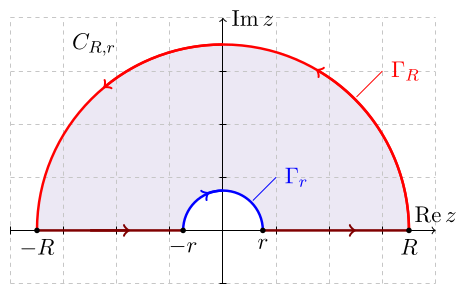
\includegraphics[width=0.7\textwidth]{images/analyse_complexe/ac-015-000.png}
\caption{Représentation d'une intégrale dans le plan complexe.}
\end{figure}

\begin{figure}[H]
\centering

\includegraphics[width=0.7\textwidth]{images/analyse_complexe/ac-015-001.png}
\caption{Contour d'intégration et pôles.}
\end{figure}

\ifdefined\inMainDoc\else\end{document}\fi
